\section{动画变换}\label{sec:动画变换}
\begin{remark}
    本节含有高级内容,第一次阅读时可以跳过。
\end{remark}

\begin{figure}[htbp]
    \centering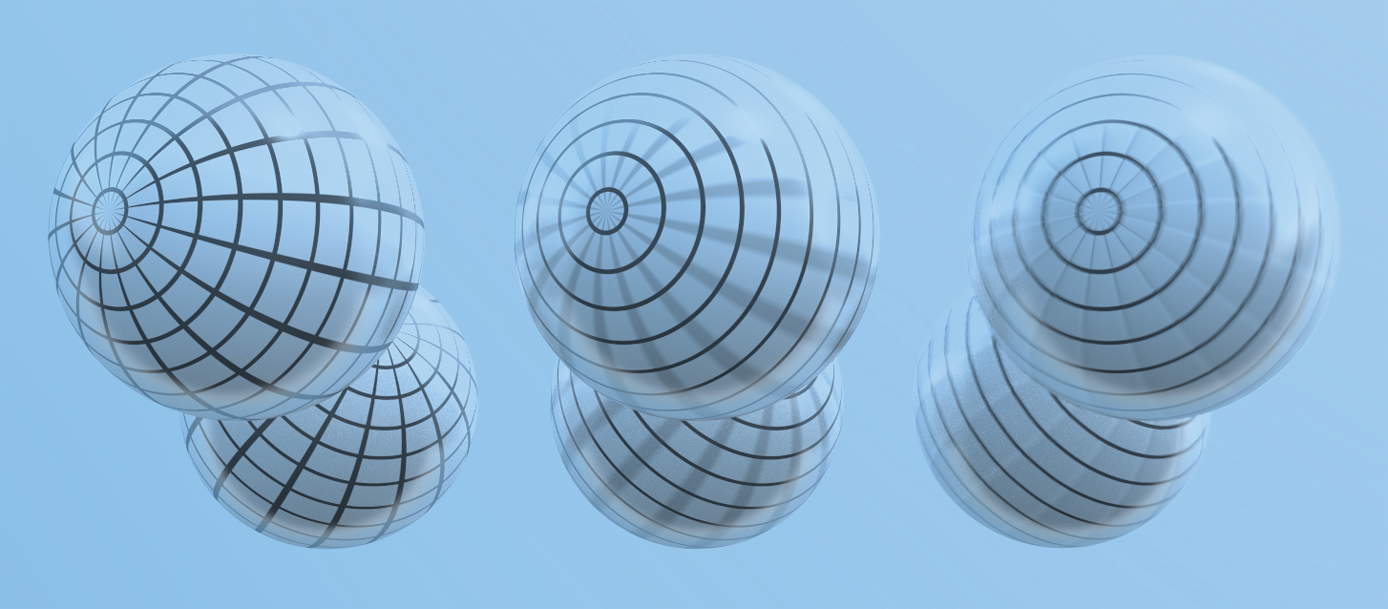
\includegraphics[width=\linewidth]{chap02/spinningspheres.png}
    \caption{转动的球体。用本节实现的变换动画代码以不同速率旋转三个球体并被镜子反射。
        注意球体的反射和球体自身一样模糊。}
    \label{fig:2.15}
\end{figure}

pbrt为场景中的相机和几何图元支持关键帧矩阵动画。
不只是提供单个变换放置场景中的相应物体,
用户还可能提供许多\keyindex{关键帧}{keyframe}{}变换,
每个都与特定时间点关联。
这能让相机移动起来并在仿真相机快门打开时让场景中的物体也移动起来。
\reffig{2.15}展示了三个运用pbrt关键帧矩阵动画的运动球体。

通常,在关键帧矩阵之间插值的问题是没有定义的。
例如,如果我们关于$x$轴旋转181度后再旋转181度,
这代表2度的小旋转还是-358度的大旋转?
再例如,考虑两个矩阵,一个是恒等的另一个是绕$z$轴旋转180度。
从其中一个到另一个有无数种方式可走。

关键帧矩阵插值在计算机动画中是一个重要的问题,
有许多不同的方法被开发出来。
幸运的是,有两个原因使得渲染器中的矩阵插值问题一般不像动画系统中的那么难。

首先,在一个像pbrt那样的渲染器中,
我们一般有分别在相机快门打开和关闭时的关键帧矩阵;
我们只需要在单张图像的时段里在两者之间插值。
在动画系统中,矩阵一般按更低的时间频率提供,
所以一对关键帧矩阵之间有许多帧;
这样,就有更多机会注意到插值中的问题。

第二,在基于物理的渲染器中,需要我们插值的矩阵对的时段越长,
虚拟相机快门就打开得越久,最终图像的运动模糊就越多;
运动模糊的增加常常隐藏了插值的缺点。

对由关键帧矩阵定义的变换最简单的插值方法——
直接对矩阵的每个分量插值——并不是一个好办法,因为它一般会导致意外不良结果。
例如,如果变换应用了不同的旋转,则即使是刚体运动,中间的矩阵也可能缩放物体,这明显不是我们期望的。
(如果矩阵在它们之间有完整180度的旋转,则插值的中间物体可能缩小到不见!)

\reffig{2.16}展示了在该帧过程中旋转90度的球体;
直接对矩阵元素插值给出的结果不如本节实现的方法准确。
\begin{figure}[htb]
    \raggedright
    \subfloat[静止球体。]{\label{fig:2.16.1}
\includegraphics[width=0.5\linewidth]{chap02/sphere-still.png}}%
    \subfloat[旋转,正确插值。]{\label{fig:2.16.2}
\includegraphics[width=0.5\linewidth]{chap02/sphere-rot-good.png}}\\%
    \subfloat[旋转,错误插值。]{\label{fig:2.16.3}
\includegraphics[width=0.5\linewidth]{chap02/sphere-rot-bad.png}}\quad%
    \begin{minipage}{0.45\textwidth}
        \vspace{-\linewidth}\caption{变换插值错误的影响。(a)球体以网格线作为纹理,没有旋转。
            (b)球体在该帧过程中旋转90度,使用本节实现的变换插值技术。
            (c)球体旋转90度,直接对矩阵分量插值来对变换插值。
            这时,动画球体错误地变大了并且靠球体外本应清晰的线条也错误地变模糊了。}
        \label{fig:2.16}
    \end{minipage}
\end{figure}

pbrt用的变换插值方法基于\keyindex{矩阵分解}{matrix decomposition}{}——
给定任意变换矩阵$\bm M$,我们将其分解为
缩放($\bm S$)、旋转($\bm R$)和平移($\bm T$)变换的级联,
\begin{align*}
    \bm M=\bm S\bm R\bm T\, ,
\end{align*}
其中这些分量每个都是独立插值,然后三个插值矩阵相乘得到合成插值矩阵。

平移和缩放的插值可以由矩阵分量的线性插值轻松准确完成;
旋转插值则更困难。
在描述pbrt中的矩阵分解实现之前,我们首先介绍\keyindex{四元数}{quaternion}{},
它对旋转的优雅表示将给出高效的插值方法。

\subsection{四元数}\label{sub:四元数}
四元数\sidenote{译者注:本节内容对四元数的介绍比较精简,不加证明地给出相关性质。
    如果你关心这些性质背后的原因是什么,可以阅读译者自行整理编写的\refsec{译者补充:四元数}。}
作为复数的推广,最初由William Rowan Hamilton爵士于1843年发明。
就像复数可以定义为实部和虚部之和$x+y\mathbf{i}$,其中$\mathbf{i}^2=-1$那样,
他确定也能推广到四维,得到了四元数。

四元数是一个四元组,
\begin{align}\label{eq:2.4}
    \bm q=[x,y,z,w]=w+x\mathbf{i}+y\mathbf{j}+z\mathbf{k}\, ,
\end{align}
其中$\mathbf{i}, \mathbf{j}, \mathbf{k}$定义
\footnote{Hamilton发现分量之间的这种关系非常有趣,
    以至于当他想到这个时立即用刀子把公式刻在了他正经过的桥上。}
为$\mathbf{i}^2=\mathbf{j}^2=\mathbf{k}^2=\mathbf{i}\mathbf{j}\mathbf{k}=-1$。
分量间的另一重要关系是$\mathbf{i}\mathbf{j}=\mathbf{k}$且
$\mathbf{j}\mathbf{i}=-\mathbf{k}$。
这说明四元数乘法一般是不可交换的。

四元数可以表示为四元组$\bm q=[q_x,q_y,q_z,q_w]$或$[\bm q_{xyz},q_w]$,
其中$\bm q_{xyz}$是虚部三维向量,$q_w$是实部。
本节中我们会穿插使用这两种表示。

两个任意四元数的乘积表达式可以通过展开它们定义的实部和虚部得到:
\begin{align*}
    \bm q\bm q'=(q_w+q_x\mathbf{i}+q_y\mathbf{j}+q_z\mathbf{k})(q'_w+q'_x\mathbf{i}+q'_y\mathbf{j}+q'_z\mathbf{k})\, .
\end{align*}

整理各项并利用像上面列出的分量间恒等式(例如$\mathbf{i}^2=-1$),
结果可用向量叉积和点积简洁地表示为
\begin{align}\label{eq:2.5}
    (\bm q\bm q')_{xyz} & =\bm q_{xyz}\times\bm q'_{xyz}+q_w\bm q'_{xyz}+q'_w\bm q_{xyz}\nonumber\, , \\
    (\bm q\bm q')_w     & =q_wq'_w-(\bm q_{xyz}\cdot\bm q'_{xyz})\, .
\end{align}

单位四元数(分量满足$x^2+y^2+z^2+w^2=1$的四元数)和
$\mathbb{R}^3$空间中的旋转之间有一很有用的关系:具体来说,
绕着可以映射为单位四元数$[\hat{\bm v}\sin\theta,\cos\theta]$的
单位轴$\hat{\bm v}$旋转角度$2\theta$时,
下列四元数乘积等效于将旋转施加到点$\bm p$后表达为齐次坐标形式:
\begin{align*}
    \bm p'=\bm q\bm p\bm q^{-1}\, .
\end{align*}

并且,若干旋转四元数的积得到的另一个四元数等价于依次施加旋转。

pbrt中文件\href{https://github.com/mmp/pbrt-v3/tree/master/src/core/quaternion.h}{{\ttfamily core/quaternion.h}}
和\href{https://github.com/mmp/pbrt-v3/tree/master/src/core/quaternion.cpp}{{\ttfamily core/quaternion.cpp}}
中有类\refvar{Quaternion}{}
的实现。默认构造函数初始化一个单位四元数。
\begin{lstlisting}
`\initcode{Quaternion Public Methods}{=}\initnext{QuaternionPublicMethods}`
`\initvar{Quaternion}{}`() : `\refvar[Quaternion::v]{v}{}`(0, 0, 0), `\refvar[Quaternion::w]{w}{}`(1) { }
\end{lstlisting}

我们用\refvar{Vector3f}{}表示四元数的$xyz$分量;
这样可以在下面一些方法的实现中利用\refvar{Vector3f}{}的各种方法。
\begin{lstlisting}
`\initcode{Quaternion Public Data}{=}`
`\refvar{Vector3f}{}` `\initvar[Quaternion::v]{v}{}`;
`\refvar{Float}{}` `\initvar[Quaternion::w]{w}{}`;
\end{lstlisting}

四元数的加减法逐元素执行。这直接由\refeq{2.4}推导而来。例如
\begin{align*}
    \bm q+\bm q' & =(w+x\mathbf{i}+y\mathbf{j}+z\mathbf{k})(w'+x'\mathbf{i}+y'\mathbf{j}+z'\mathbf{k})\nonumber \\
                 & =(w+w')+(x+x')\mathbf{i}+(y+y')\mathbf{j}+(z+z')\mathbf{k}\, .
\end{align*}

其他算术方法(减法、乘法以及除以标量)也有类似定义和实现,此处不再赘述。
\begin{lstlisting}
`\refcode{Quaternion Public Methods}{+=}\lastnext{QuaternionPublicMethods}`
`\refvar{Quaternion}{}` &operator+=(const `\refvar{Quaternion}{}` &q) {
    `\refvar[Quaternion::v]{v}{}` += q.`\refvar[Quaternion::v]{v}{}`;
    `\refvar[Quaternion::w]{w}{}` += q.`\refvar[Quaternion::w]{w}{}`;
    return *this;
}
\end{lstlisting}

两个四元数的内积由方法\refvar[Quaternion::Dot]{Dot}{()}实现,
并且四元数可以被它的长度规范化。
\begin{lstlisting}
`\initcode{Quaternion Inline Functions}{=}\initnext{QuaternionInlineFunctions}`
inline `\refvar{Float}{}` `\initvar[Quaternion::Dot]{Dot}{}`(const `\refvar{Quaternion}{}` &q1, const `\refvar{Quaternion}{}` &q2) {
    return `\refvar{Dot}{}`(q1.`\refvar[Quaternion::v]{v}{}`, q2.`\refvar[Quaternion::v]{v}{}`) + q1.`\refvar[Quaternion::w]{w}{}` * q2.`\refvar[Quaternion::w]{w}{}`;
}
\end{lstlisting}

\begin{lstlisting}
`\refcode{Quaternion Inline Functions}{+=}\lastcode{QuaternionInlineFunctions}`
inline `\refvar{Quaternion}{}` `\initvar[Quaternion::Normalize]{Normalize}{}`(const `\refvar{Quaternion}{}` &q) {
    return q / std::sqrt(`\refvar[Quaternion::Dot]{Dot}{}`(q, q));
}
\end{lstlisting}

能够计算和四元数表示同一旋转的变换矩阵非常有用。特别地,在类
\refvar{AnimatedTransform}{}中用四元数对旋转插值后,
我们需要将插值后的旋转转换回变换矩阵来计算最后合成的插值矩阵。

为了推导四元数的旋转矩阵,回忆一下四元数对点的变换由$\bm q\bm p\bm q^{-1}$给出。
我们想要矩阵$\bm M$执行相同的变换,即$\bm p'=\bm M\bm p$。
如果我们用\refeq{2.5}展开四元数乘法$\bm q\bm p\bm q^{-1}$、
用四元数基本恒等式化简、合并项并把结果表示为矩阵,
我们可以得到如下$3\times3$矩阵表示同一变换:
\begin{align}\label{eq:2.6}
    \bm M=\left[
        \begin{array}{ccc}
            1-2(q_y^2+q_z^2) & 2(q_xq_y+q_zq_w) & 2(q_xq_z-q_yq_w) \\
            2(q_xq_y-q_zq_w) & 1-2(q_x^2+q_z^2) & 2(q_yq_z+q_xq_w) \\
            2(q_xq_z+q_yq_w) & 2(q_yq_z-q_xq_w) & 1-2(q_x^2+q_y^2)
        \end{array}
        \right]\, .
\end{align}

该计算由方法\refvar[ToTransform]{Quaternion::ToTransform}{()}实现。
我们此处不介绍它的实现,因为它就是\refeq{2.6}的直接实现。
\begin{lstlisting}
`\refcode{Quaternion Public Methods}{+=}\lastnext{QuaternionPublicMethods}`
`\refvar{Transform}{}` `\initvar{ToTransform}{}`() const;
\end{lstlisting}

注意我们可以利用一个单位四元数
$\displaystyle[\bm q_{xyz}\sin\frac{\theta}{2},\cos\frac{\theta}{2}]$表示
绕单位轴$\hat{\bm q}_{xyz}$旋转角度$\theta$的事实计算旋转矩阵。
首先我们计算出旋转角度为$\theta=2\arccos q_w$,
然后利用之前定义的函数\refvar{Rotate}{()},
传入轴$\hat{\bm q}_{xyz}$和旋转角度$\theta$。
然而,这个替代方法会很低效,因为需要多次调用三角函数,
但是这里实现的方法只用了浮点加法、减法和乘法。

从旋转矩阵创建四元数也很有用。
为此,\refvar{Quaternion}{}提供了接收\refvar{Transform}{}
的构造函数。合适的四元数可以通过利用\refeq{2.6}中旋转矩阵元素与四元数分量之间的关系算得。
例如,如果我们从矩阵本身中减去它的转置,则结果矩阵的$(0,1)$分量为$-4q_wq_z$。
因此,给定已知值的特定旋转矩阵实例,
可以利用矩阵值与四元数分量之间大量这样的关系生成一系列可以求解四元数分量的方程。

本文中我们不介绍推导细节或实际实现
\sidenote{译者注:笔者将其补充到了\refsub{四元数与旋转变换}。};
关于怎样推导这项技术的更多信息,
包括处理数值稳定性,详见\citet{SHOEMAKE1991351}。

\begin{lstlisting}
`\refcode{Quaternion Public Methods}{+=}\lastcode{QuaternionPublicMethods}`
`\refvar{Quaternion}{}`(const `\refvar{Transform}{}` &t);
\end{lstlisting}

\subsection{四元数插值}\label{sub:四元数插值}
我们最后要定义的函数\refvar{Slerp}{()},
在两个四元数之间进行\keyindex{球面线性插值}{spherical linear interpolation}{interpolation插值}(slerp)。
球面线性插值可在球体表面大圆的弧线上做匀速率运动,
因此对于旋转插值有两个期望的性质:
\begin{itemize}
    \item 旋转插值路径使得\keyindex{扭矩最小化}{torque minimization}{}:
          两个旋转之间所得路径是旋转空间中所能得到的最短路径。
    \item 插值有\keyindex{恒定角速度}{constant angular velocity}{}:
          动画参数{\ttfamily t}的变化量和所得旋转的变化量的关系在插值过程中是恒定的
          (换句话说,在插值范围内,插值速度是恒定的)。
\end{itemize}

参考本章末“扩展阅读”一节更彻底地讨论好的旋转插值该有什么性质。

如下的四元数球面线性插值最初由\citet{10.1145/325334.325242}提出,
给定两个四元数$\bm q_1$和$\bm q_2$和参数值$t\in[0,1]$以在两者之间插值
\sidenote{译者注:利用三角形的正弦定理可以推导出该公式。}:
\begin{align*}
    \mathrm{slerp}(\bm q_1,\bm q_2,t)=\frac{\bm q_1\sin((1-t)\theta)+\bm q_2\sin(t\theta)}{\sin\theta}\, .
\end{align*}

\citet{Blow_2004}提出了一种直观的方式理解\refvar{Slerp}{()}。
下文中,给定要在其间插值的四元数$\bm q_1$和$\bm q_2$,两者角度记为$\theta$。
然后,给定参数值$t\in[0,1]$,我们想要找到中间的四元数$\bm q'$使得
它沿从$\bm q_1$到$\bm q_2$的路径与$\bm q_1$的角度为$\theta'=\theta t$。

\begin{figure}[htbp]
    \centering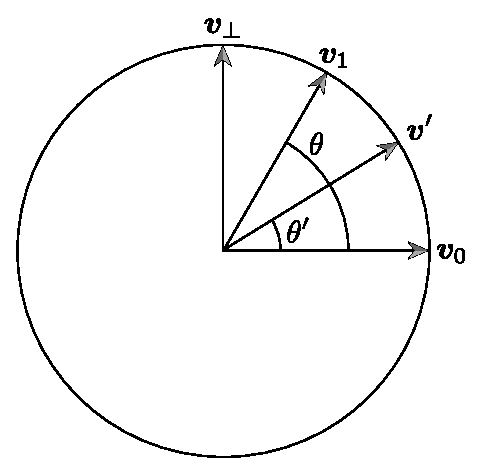
\includegraphics[scale=0.6]{chap02/Quaternionrotation.eps}
    \caption{为了理解四元数球面线性插值,考虑2D下的两个单位圆上的向量$\bm v_0$和$\bm v_1$,
        两者夹角$\theta$。我们想要计算两者间角度为$\theta'$的插值向量。
        为此,我们可以寻找正交于$\bm v_0$的向量$\bm v_{\perp}$,
        再应用三角恒等式$\bm v'=\bm v_0\cos\theta'+\bm v_{\perp}\sin\theta'$。}
    \label{fig:2.17}
\end{figure}

一个计算$\bm q'$的简单方法是先在四元数空间中计算一个正交坐标系,
一个轴为$\bm q_1$,另一个是与$\bm q_1$正交的四元数,
这样两轴就构成张开$\bm q_1$和$\bm q_2$的基。

有了这个坐标系,我们就能计算关于$\bm q_1$的旋转
(见\reffig{2.17}展示的2D设置下的概念)。
正交向量$\bm q_{\perp}$可以通过将$\bm q_2$投影到$\bm q_1$并
从$\bm q_2$减去该正交投影得到;
剩余部分保证与$\bm q_1$正交:
\begin{align}\label{eq:2.7}
    \bm q_{\perp}=\bm q_2-(\bm q_1\cdot\bm q_2)\bm q_1\, .
\end{align}
给定坐标系和规范化的$\bm q_{\perp}$,沿动画路径的四元数为
\begin{align}\label{eq:2.8}
    \bm q'=\bm q_1\cos(\theta t)+\hat{\bm q}_{\perp}\sin(\theta t)\, .
\end{align}

函数\refvar{Slerp}{()}的实现检查看两个四元数是否几乎平行,
是的话它就按顺序对四元数分量用普通的线性插值以避免数值不稳定。
否则,它就用\refeq{2.7}计算正交四元数{\ttfamily qperp},
然后按\refeq{2.8}计算插值的四元数。
\begin{lstlisting}
`\initcode{Quaternion Method Definitions}{=}`
`\refvar{Quaternion}{}` `\initvar{Slerp}{}`( `\refvar{Float}{}` t, const `\refvar{Quaternion}{}` &q1,
                 const `\refvar{Quaternion}{}` &q2) {
     `\refvar{Float}{}` cosTheta = `\refvar[Quaternion::Dot]{Dot}{}`(q1, q2);
    if (cosTheta > .9995f)
        return `\refvar[Quaternion::Normalize]{Normalize}{}`((1 - t) * q1 + t * q2);
    else {
        `\refvar{Float}{}` theta = std::acos(`\refvar{Clamp}{}`(cosTheta, -1, 1));
        `\refvar{Float}{}` thetap = theta * t;
        `\refvar{Quaternion}{}` qperp = `\refvar[Quaternion::Normalize]{Normalize}{}`(q2 - q1 * cosTheta);
        return q1 * std::cos(thetap) + qperp * std::sin(thetap);
    }
}
\end{lstlisting}

\subsection{动画变换实现}\label{sub:动画变换实现}
有了四元数基础知识,我们现在就能实现类\refvar{AnimatedTransform}{}了,
它在pbrt中实现关键帧变换的插值。
其构造函数接收两个变换以及关联的时间值。

正如之前提到的,\refvar{AnimatedTransform}{}将
给定的合成变换矩阵分解为缩放、旋转和平移分量。
分解由方法\refvar[Decompose]{AnimatedTransform::Decompose}{()}执行。

\begin{lstlisting}
`\initcode{AnimatedTransform Method Definitions}{=}\initnext{AnimatedTransformMethodDefinitions}`
`\initvar{AnimatedTransform}{}`::`\refvar{AnimatedTransform}{}`(const `\refvar{Transform}{}` *startTransform,
        `\refvar{Float}{}` startTime, const `\refvar{Transform}{}` *endTransform, `\refvar{Float}{}` endTime)
    : `\refvar{startTransform}{}`(startTransform), `\refvar{endTransform}{}`(endTransform),
      `\refvar{startTime}{}`(startTime), `\refvar{endTime}{}`(endTime),
      `\refvar{actuallyAnimated}{}`(*startTransform != *endTransform) {
    `\refvar{Decompose}{}`(startTransform->m, &`\refvar[AnimatedTransform::T]{T}{}`[0], &`\refvar[AnimatedTransform::R]{R}{}`[0], &`\refvar[AnimatedTransform::S]{S}{}`[0]);
    `\refvar{Decompose}{}`(endTransform->m, &`\refvar[AnimatedTransform::T]{T}{}`[1], &`\refvar[AnimatedTransform::R]{R}{}`[1], &`\refvar[AnimatedTransform::S]{S}{}`[1]);
    `\refcode{Flip R[1] if needed to select shortest path}{}`
    `\refvar{hasRotation}{}` = `\refvar[Quaternion::Dot]{Dot}{}`(`\refvar[AnimatedTransform::R]{R}{}`[0], `\refvar[AnimatedTransform::R]{R}{}`[1]) < 0.9995f;
    `\initcode{Compute terms of motion derivative function}{}`
}
\end{lstlisting}

\begin{lstlisting}
`\initcode{AnimatedTransform Private Data}{=}\initnext{AnimatedTransformPrivateData}`
const `\refvar{Transform}{}` *`\initvar{startTransform}{}`, *`\initvar{endTransform}{}`;
const `\refvar{Float}{}` `\initvar{startTime}{}`, `\initvar{endTime}{}`;
const bool `\initvar{actuallyAnimated}{}`;
`\refvar{Vector3f}{}` `\initvar[AnimatedTransform::T]{T}{}`[2];
`\refvar{Quaternion}{}` `\initvar[AnimatedTransform::R]{R}{}`[2];
`\refvar{Matrix4x4}{}` `\initvar[AnimatedTransform::S]{S}{}`[2];
bool `\initvar{hasRotation}{}`;
\end{lstlisting}

给定一变换的合成矩阵,关于合成它的任何单个变换的信息已经损失了。
例如,给定一先平移再缩放的矩阵乘积,
一个等价矩阵也可以是先缩放再平移(但量不同)。
因此,我们需要为分解选择一个标准变换序列。
此处根据我们的需要,具体选哪个并不重要
(例如在动画系统中这会更重要因为它要分解合成矩阵使其可编辑改变独立分量)。

我们这里只处理\keyindex{仿射变换}{affine transformation}{transformation变换},
渲染系统中的动画相机和几何图元都需要它;
透视变换一般与这样的物体动画无关。

我们将使用下列变换分解:
\begin{align}\label{eq:2.9}
    \bm M=\bm T\bm R\bm S\, ,
\end{align}
其中$\bm M$是给定变换,$\bm T$是平移,$\bm R$是旋转,$\bm S$是缩放。
$\bm S$实际上是一种表示在\emph{某些}坐标系下的通用缩放
(Shoemake和Duff称之为拉伸\sidenote{译者注:原文stretch。}),
而不一定在是当前坐标系下。
不论哪种情况,它都仍然可以按分量正确地线性插值。
给定\refvar{Matrix4x4}{},方法\refvar{Decompose}{()}计算其分解。
\begin{lstlisting}
`\refcode{AnimatedTransform Method Definitions}{+=}\lastnext{AnimatedTransformMethodDefinitions}`
void `\refvar{AnimatedTransform}{}`::`\initvar{Decompose}{}`(const `\refvar{Matrix4x4}{}` &m, `\refvar{Vector3f}{}` *T,
        `\refvar{Quaternion}{}` *Rquat, `\refvar{Matrix4x4}{}` *S) {
    `\refcode{Extract translation T from transformation matrix}{}`
    `\refcode{Compute new transformation matrix M without translation}{}`
    `\refcode{Extract rotation R from transformation matrix}{}`
    `\refcode{Compute scale S using rotation and original matrix}{}`
}
\end{lstlisting}

提取平移$\bm T$很简单;
可直接从变换矩阵适当的$1\times4$元素中找到它。
\begin{lstlisting}
`\initcode{Extract translation T from transformation matrix}{=}`
T->x = m.`\refvar[Matrix4x4::m]{m}{}`[0][3];
T->y = m.`\refvar[Matrix4x4::m]{m}{}`[1][3];
T->z = m.`\refvar[Matrix4x4::m]{m}{}`[2][3];
\end{lstlisting}

既然我们假设是仿射变换(没有透视分量),
我们可以去掉平移,剩下上面表示缩放和旋转的$3\times3$矩阵。
该矩阵被复制到新矩阵{\ttfamily M}中做进一步处理。
\begin{lstlisting}
`\initcode{Compute new transformation matrix M without translation}{=}`
`\refvar{Matrix4x4}{}` M = m;
for (int i = 0; i < 3; ++i)
    M.`\refvar[Matrix4x4::m]{m}{}`[i][3] = M.`\refvar[Matrix4x4::m]{m}{}`[3][i] = 0.f;
M.`\refvar[Matrix4x4::m]{m}{}`[3][3] = 1.f;
\end{lstlisting}

接着我们想提取纯旋转分量$\bm R$。
我们使用称为\keyindex{极分解}{polar decomposition}{}的技术来完成它。
可以证明矩阵$\bm M$极分解为旋转$\bm R$和缩放$\bm S$可以通过
依次平均$\bm M$和它的逆转置算得
\begin{align}\label{eq:2.10}
    \bm M_{i+1}=\frac{1}{2}(\bm M_i+(\bm M_i^\mathrm{T})^{-1})\, ,
\end{align}
直到收敛于点$\bm M_i=\bm R$。
(容易看到如果$\bm M$是纯旋转,则平均它及其逆转置会保持不变,
因为它的逆等于转置。“扩展阅读”一节有更多讨论
为什么该序列收敛于原始变换旋转分量的参考文献。)
\citet{10.5555/155294.155324}证明
结果矩阵是最接近$\bm M$的正交矩阵——我们期望的性质
\sidenote{译者注:笔者将这部分内容整理为补充的\refsec{译者补充:分解旋转矩阵}。}。

为了计算该序列,我们迭代应用\refeq{2.10}直到相邻两项之间的差很小或
执行了固定数目的循环。
实际上,该序列一般收敛得很快。
\begin{lstlisting}
`\initcode{Extract rotation R from transformation matrix}{=}`
`\refvar{Float}{}` norm;
int count = 0;
`\refvar{Matrix4x4}{}` R = M;
do {
    `\refcode{Compute next matrix Rnext in series}{}`
    `\refcode{Compute norm of difference between R and Rnext}{}`
    R = Rnext;
} while (++count < 100 && norm > .0001);
*Rquat = `\refvar{Quaternion}{}`(R);
\end{lstlisting}
\begin{lstlisting}
`\initcode{Compute next matrix Rnext in series}{=}`
`\refvar{Matrix4x4}{}` Rnext;
`\refvar{Matrix4x4}{}` Rit = `\refvar[Matrix4x4::Inverse]{Inverse}{}`(`\refvar[Matrix4x4::Transpose]{Transpose}{}`(R));
for (int i = 0; i < 4; ++i)
    for (int j = 0; j < 4; ++j)
        Rnext.`\refvar[Matrix4x4::m]{m}{}`[i][j] = 0.5f * (R.`\refvar[Matrix4x4::m]{m}{}`[i][j] + Rit.`\refvar[Matrix4x4::m]{m}{}`[i][j]);
\end{lstlisting}
\begin{lstlisting}
`\initcode{Compute norm of difference between R and Rnext}{=}`
norm = 0;
for (int i = 0; i < 3; ++i) {
    `\refvar{Float}{}` n = std::abs(R.`\refvar[Matrix4x4::m]{m}{}`[i][0] - Rnext.`\refvar[Matrix4x4::m]{m}{}`[i][0]) + 
              std::abs(R.`\refvar[Matrix4x4::m]{m}{}`[i][1] - Rnext.`\refvar[Matrix4x4::m]{m}{}`[i][1]) + 
              std::abs(R.`\refvar[Matrix4x4::m]{m}{}`[i][2] - Rnext.`\refvar[Matrix4x4::m]{m}{}`[i][2]);
    norm = std::max(norm, n);
}
\end{lstlisting}

一旦我们从$\bm M$提取了旋转,剩下的全部就是缩放了。
我们想寻找满足$\bm M=\bm R\bm S$的矩阵$\bm S$。
现在我们知道了$\bm R$和$\bm M$,只需解得$\bm S=\bm R^{-1}\bm M$。
\begin{lstlisting}
`\initcode{Compute scale S using rotation and original matrix}{=}`
*S = `\refvar{Matrix4x4::Mul}{}`(`\refvar[Matrix4x4::Inverse]{Inverse}{}`(R), M);
\end{lstlisting}

对于每个旋转矩阵,有两个单位四元数与其矩阵对应且只相差一个符号。
如果我们提取到的两个旋转的点积是负数,则两者之间的slerp不会
在相应的两个旋转之间走最短路径。
令其中一个取负(这里即任意选择第二个)可以改为取到最短路径。
\begin{lstlisting}
`\initcode{Flip R[1] if needed to select shortest path}{=}`
if (`\refvar{Dot}{}`(`\refvar[AnimatedTransform::R]{R}{}`[0], `\refvar[AnimatedTransform::R]{R}{}`[1]) < 0)
    `\refvar[AnimatedTransform::R]{R}{}`[1] = -`\refvar[AnimatedTransform::R]{R}{}`[1];
\end{lstlisting}

方法\refvar{Interpolate}{()}计算给定时刻的插值变换矩阵。
通过插值之前提取的平移、旋转和缩放再相乘得到
表示三种变换综合效应的合成矩阵。
\begin{lstlisting}
`\refcode{AnimatedTransform Method Definitions}{+=}\lastnext{AnimatedTransformMethodDefinitions}`
void `\refvar{AnimatedTransform}{}`::`\initvar{Interpolate}{}`(`\refvar{Float}{}` time, `\refvar{Transform}{}` *t) const {
    `\refcode{Handle boundary conditions for matrix interpolation}{}`
    `\refvar{Float}{}` dt = (time - `\refvar{startTime}{}`) / (`\refvar{endTime}{}` - `\refvar{startTime}{}`);
    `\refcode{Interpolate translation at dt}{}`
    `\refcode{Interpolate rotation at dt}{}`
    `\refcode{Interpolate scale at dt}{}`
    `\refcode{Compute interpolated matrix as product of interpolated components}{}`
}
\end{lstlisting}

如果给定时间值超出存于\refvar{AnimatedTransform}{}的两个变换的时间范围,
则视情况返回开始或结束时刻的变换。
\refvar{AnimatedTransform}{}构造函数也检查两个\refvar{Transform}{}是否相同;
如果是,则没有必要插值。
pbrt中所有支持动画的类都永远为其变换保存了\refvar{AnimatedTransform}{},
而不是视情况保存\refvar{Transform}{}或
\refvar{AnimatedTransform}{}。
尽管确实值得检查这种情况而不必要在两个相等的变换之间插值,
但这简化了它们的实现。
\begin{lstlisting}
`\initcode{Handle boundary conditions for matrix interpolation}{=}`
if (!`\refvar{actuallyAnimated}{}` || time <= `\refvar{startTime}{}`) { 
    *t = *`\refvar{startTransform}{}`;
    return; 
}
if (time >= `\refvar{endTime}{}`) { 
    *t = *`\refvar{endTransform}{}`;
    return; 
}
\end{lstlisting}

变量{\ttfamily dt}保存了从\refvar{startTime}{}到\refvar{endTime}{}范围的偏移量;
在\refvar{startTime}{}处取零,\refvar{endTime}{}处取一。
给定{\ttfamily dt},平移的插值很简单。
\begin{lstlisting}
`\initcode{Interpolate translation at dt}{=}`
`\refvar{Vector3f}{}` trans = (1 - dt) * `\refvar[AnimatedTransform::T]{T}{}`[0] + dt * `\refvar[AnimatedTransform::T]{T}{}`[1];
\end{lstlisting}

开始和结束之间的旋转插值用\refvar{Slerp}{()}例程(\refsub{四元数插值})。
\begin{lstlisting}
`\initcode{Interpolate rotation at dt}{=}`
`\refvar{Quaternion}{}` rotate = `\refvar{Slerp}{}`(dt, `\refvar[AnimatedTransform::R]{R}{}`[0], `\refvar[AnimatedTransform::R]{R}{}`[1]);
\end{lstlisting}

最后,缩放插值矩阵通过对开始和结束缩放矩阵的独立分量插值算得。
因为\refvar{Matrix4x4}{}构造函数把矩阵设置为单位矩阵,
我们不需要初始化{\ttfamily scale}的其他任何元素。
\begin{lstlisting}
`\initcode{Interpolate scale at dt}{=}`
`\refvar{Matrix4x4}{}` scale;
for (int i = 0; i < 3; ++i)
    for (int j = 0; j < 3; ++j)
        scale.m[i][j] = `\refvar{Lerp}{}`(dt, `\refvar[AnimatedTransform::S]{S}{}`[0].m[i][j], `\refvar[AnimatedTransform::S]{S}{}`[1].m[i][j]);
\end{lstlisting}

有了三个插值部分,它们三个变换矩阵的积就给出了最后的结果。
\begin{lstlisting}
`\initcode{Compute interpolated matrix as product of interpolated components}{=}`
*t = `\refvar{Translate}{}`(trans) * rotate.`\refvar{ToTransform}{}`() * `\refvar{Transform}{}`(scale);
\end{lstlisting}

\refvar{AnimatedTransform}{}也用\refvar{Point3f}{}和
\refvar{Vector3f}{}的时间以及\refvar{Ray}{}的\refvar{Ray::time}{}
来提供大量直接应用插值变换的方法。
当实际上没有动画时,这些方法比调用\refvar[Interpolate]{AnimatedTransform::Interpolate}{()}再
使用返回的矩阵更高效,因为那种情况下不需要复制变换矩阵。
\begin{lstlisting}
`\initcode{AnimatedTransform Public Methods}{=}`
`\refvar{Ray}{}` operator()(const `\refvar{Ray}{}` &r) const;
`\refvar{RayDifferential}{}` operator()(const `\refvar{RayDifferential}{}` &r) const;
`\refvar{Point3f}{}` operator()(`\refvar{Float}{}` time, const `\refvar{Point3f}{}` &p) const;
`\refvar{Vector3f}{}` operator()(`\refvar{Float}{}` time, const `\refvar{Vector3f}{}` &v) const;
\end{lstlisting}

\subsection{定界移动边界框}\label{sub:定界移动边界框}
给定经过动画变换的\refvar{Bounds3f}{},
计算包围了动画时段里全部运动的边界框很有用。
例如,如果我们能定界动画几何图元的运动,
我们就能在按光线时间插值图元边界以检查相交性并承担开销之前,
用光线与该边界的相交性来确定光线是否会与物体相交。
方法\refvar[MotionBounds]{AnimatedTransform::MotionBounds}{()}
执行该运算,接收边界框并返回\refvar{AnimatedTransform}{}时间段内其运动的边界框。

有两种简单情况:第一,如果关键帧矩阵相等,
则我们可以任意地只施加开始的变换来计算完整边框。
第二,如果变换只包括缩放和/或平移,
则包围了边界框在开始和结束时刻变换位置的边界框将包围所有运动。
为了理解为什么会这样,将变换的点$\bm p$考虑为时间的函数;
我们将其记为两个矩阵、一个点和时间的函数$a(\bm M_0,\bm M_1,\bm p,t)$。

因为这种情况下分解的旋转分量是恒等变换,所以我们将矩阵分解为:
\begin{align*}
    a(\bm M_0,\bm M_1,\bm p,t)=\bm T(t)\bm S(t)\bm p\, ,
\end{align*}
其中平移和缩放都写作时间的函数。
为了简便,假设$\bm S(t)$是常规缩放,
我们可以求得$a(\bm M_0,\bm M_1,\bm p,t)$的分量表达式。
例如,对于$x$分量有
\begin{align*}
    a(\bm M_0,\bm M_1,\bm p,t)_x & =((1-t)s_{0,0}+ts'_{0,0})p_x+(1-t)d_{0,3}+td'_{0,3}                \\
                                 & =(s_{0,0}+d_{0,3})+(-s_{0,0}p_x+s'_{0,0}p_x-d_{0,3}+d'_{0,3})t\, ,
\end{align*}
其中$s_{0,0}$是缩放矩阵$\bm M_0$的相应元素,同样$s'_{0,0}$是缩放矩阵$\bm M_1$的元素,
平移矩阵的元素类似地表示为$d$(这里我们用$d$表示“delta”,因为$t$已经用来表示时间了)。
作为$t$的线性函数,该函数的极值在开始和结束时刻取得。
对于一般缩放下的其他坐标和情况也有类似结论。
\begin{lstlisting}
`\refcode{AnimatedTransform Method Definitions}{+=}\lastnext{AnimatedTransformMethodDefinitions}`
`\refvar{Bounds3f}{}` `\refvar{AnimatedTransform}{}`::`\initvar{MotionBounds}{}`(const `\refvar{Bounds3f}{}` &b) const {
    if (!`\refvar{actuallyAnimated}{}`)
        return (*`\refvar{startTransform}{}`)(b);
    if (`\refvar{hasRotation}{}` == false)
        return `\refvar[Union2]{Union}{}`((*`\refvar{startTransform}{}`)(b), (*`\refvar{endTransform}{}`)(b));
    `\refcode{Return motion bounds accounting for animated rotation}{}`
}
\end{lstlisting}

对于有动画旋转的一般情况,运动函数可能在时间段中间有极值。
我们不知道寻找这些点的简单方法。
许多渲染器通过在时间段内采样大量时间点、
在每一点计算插值变换、再取所有相应变换后的边界框的并集来解决该问题。
这里我们开发了一种更理性的方法使得我们可以稳定地计算这些运动的边界。

我们使用稍微简单的保守边界,即需要分别计算边界框八个顶点的运动
并寻找它们边界的并集。
\begin{lstlisting}
`\initcode{Return motion bounds accounting for animated rotation}{=}`
`\refvar{Bounds3f}{}` bounds;
for (int corner = 0; corner < 8; ++corner)
    bounds = `\refvar[Union1]{Union}{}`(bounds, `\refvar{BoundPointMotion}{}`(b.`\refvar{Corner}{}`(corner)));
return bounds;
\end{lstlisting}

对于每个边界框顶点$\bm p$,我们需要寻找$a$在整个动画时间段上的极值。
回想微积分中闭区间上连续函数的极值要么在边界点要么在一阶导数为零的点。
因此,总边界由运动开始和结束时的位置以及任何极值位置的并集给出。

对于某点所关注的运动路径,\reffig{2.18}展示了运动函数的一个坐标及其导数的图示。
注意函数在整个时间段上的最大值在导数为零的点取得。
\begin{figure}[htbp]
    \centering
    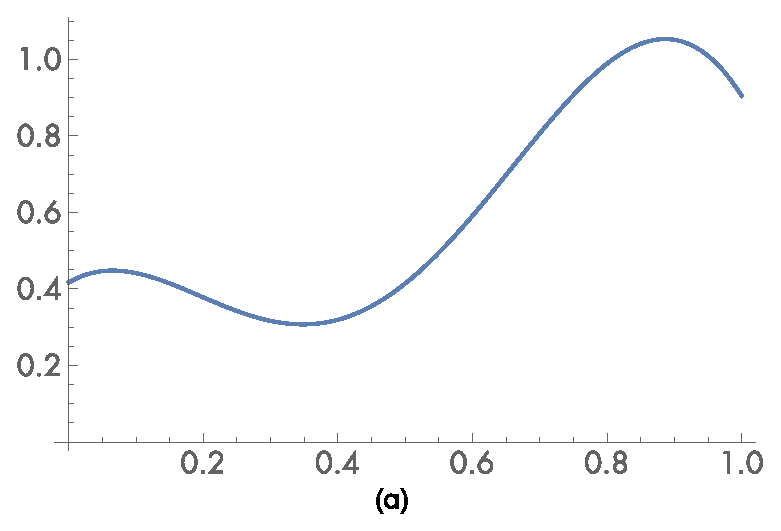
\includegraphics[scale=0.5]{chap02/point-motion.eps}
    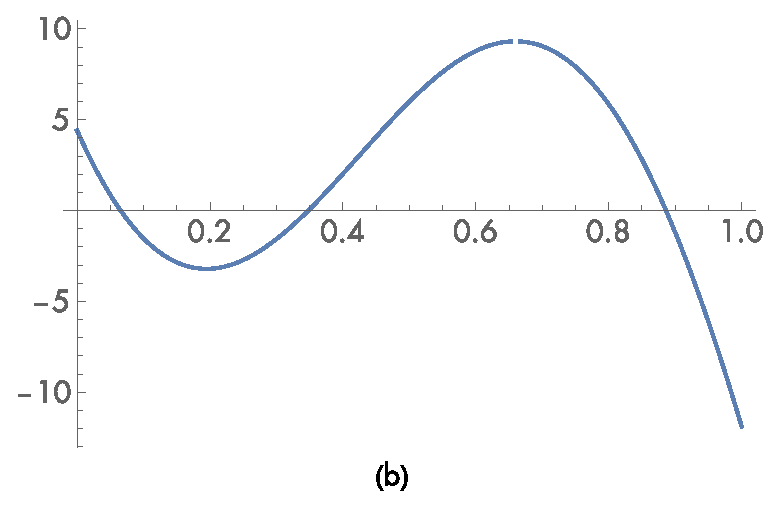
\includegraphics[scale=0.5]{chap02/point-motion-deriv.eps}
    \caption{(a)点$\bm p$的$x$坐标的运动是时间的函数,由两个关键帧矩阵决定。
        (b)运动函数的导数,\refeq{2.12}。注意给定时间范围内运动函数的极值对应导数的零点。}
    \label{fig:2.18}
\end{figure}

为了定界单点的运动,我们用下面无旋转情况的方法开始推导,
将\refeq{2.9}的三个分量$\bm T,\bm R$和$\bm S$展开为时间的函数并
求它们的积。我们得到:
\begin{align}\label{eq:2.11}
    a(\bm M_0,\bm M_1,\bm p,t)=\bm T(t)\bm R(t)\bm S(t)\bm p\, .
\end{align}
结果展开会非常复杂,绝大多数是slerp和四元数转换为矩阵的结果造成的;
需要计算机代数系统才能处理该函数。

导数$\displaystyle\frac{\partial}{\partial t}a(\bm M_0,\bm M_1,\bm p,t)$也相当复杂——
它的完整代数运算非常壮观,
对于给定的一对分解的矩阵、点和时间,需要两千多次运算才能求值。
然而,对于特定的变换矩阵和特定点,$a$可以大大简化;
我们把专门关于$t$的函数表示为$a_{\bm M,\bm p}(t)$。
对每个坐标\sidenote{译者注:$b_i$表示不含$t$的系数。
缩放变换后每维坐标为$b_1t+b_2$;
旋转相应的四元数各分量为$b_3\sin(\theta t)+b_4\cos(\theta t)$,
而$\bm R(t)$元素只含其二次项
$b_5\sin^2(\theta t)+b_6\cos^2(\theta t)+b_7\sin(\theta t)\cos(\theta t)$,即
$b_8+b_9\sin(2\theta t)+b_{10}\cos(2\theta t)$,故坐标旋转为
$(b_8+b_9\sin(2\theta t)+b_{10}\cos(2\theta t))(b_1t+b_2)$;$\bm T(t)$再加上$t$的一次式得
$(b_8+b_9\sin(2\theta t)+b_{10}\cos(2\theta t))(b_1t+b_2)+b_{11}t+b_{12}$。
对$t$求导即形如\refeq{2.12}。}
求导数大约要十次浮点运算、一次正弦和一次余弦:
\begin{align}\label{eq:2.12}
    \frac{\mathrm{d}a_{\bm M,\bm p}(t)}{\mathrm{d}t}=\bm c_1+(\bm c_2+\bm c_3t)\cos(2\theta t)+(\bm c_4+\bm c_5t)\sin(2\theta t)\, ,
\end{align}

其中$\theta$是两个四元数点积的反余弦,
五个系数$\bm c_i$是依赖于两个矩阵和位置$\bm p$的三维向量
\sidenote{译者注:本应是四维的齐次表达式,
    但因为平移、旋转和缩放均不改变第四维权重,
    对时间的导数恒为零,所以省略为三维向量。}。
该特殊化解决得不错,因为我们需要在许多时间点上对给定点计算该函数值。

我们现在有两项任务:第一,给定一对关键帧矩阵和一点$\bm p$,
我们首先需要能够高效计算出系数$\bm c_i$的值。
然后,有了由$\bm p$和$\bm c_i$定义的相对简单的函数,
我们需要求得\refeq{2.12}的零点,即可能代表运动极值出现的时间。

对于第一项任务,假设对于每一对关键帧矩阵都计算多点运动的边界框(即此处的情况),
我们先把对系数的贡献分为依赖于关键帧矩阵和依赖于点$\bm p$的部分
\sidenote{译者注:这句不确定翻译正确。}。
幸运的是结果很简单——向量$\bm c_i$是点的$x,y$和$z$分量的线性函数
\sidenote{译者注:为了前后文一致该式改成了向量形式(粗体),
    原文为标量形式,但本质含义一致。}。
\begin{align*}
    \bm c_i(\bm p)=\bm k_{i,c}+\bm k_{i,x}p_x+\bm k_{i,y}p_y+\bm k_{i,z}p_z\, .
\end{align*}

因此,给定系数$\bm k_i$和我们想定界其运动的特定点$\bm p$,
我们可以高效计算\refeq{2.12}中导函数的系数$\bm c_i$。
结构体\refvar{DerivativeTerm}{}封装了这些系数和计算。
\begin{lstlisting}
`\refcode{AnimatedTransform Private Data}{+=}\lastnext{AnimatedTransformPrivateData}`
struct `\initvar{DerivativeTerm}{}` {
    `\refvar{DerivativeTerm}{}`(`\refvar{Float}{}` c, `\refvar{Float}{}` x, `\refvar{Float}{}` y, `\refvar{Float}{}` z)
        : `\refvar[DerivativeTerm::kc]{kc}{}`(c), `\refvar[DerivativeTerm::kx]{kx}{}`(x), `\refvar[DerivativeTerm::ky]{ky}{}`(y), `\refvar[DerivativeTerm::kz]{kz}{}`(z) { }
    `\refvar{Float}{}` `\initvar[DerivativeTerm::kc]{kc}{}`, `\initvar[DerivativeTerm::kx]{kx}{}`, `\initvar[DerivativeTerm::ky]{ky}{}`, `\initvar[DerivativeTerm::kz]{kz}{}`;
    `\refvar{Float}{}` `\initvar[DerivativeTerm::Eval]{Eval}{}`(const `\refvar{Point3f}{}` &p) const {
        return `\refvar[DerivativeTerm::kc]{kc}{}` + `\refvar[DerivativeTerm::kx]{kx}{}` * p.x + `\refvar[DerivativeTerm::ky]{ky}{}` * p.y + `\refvar[DerivativeTerm::kz]{kz}{}` * p.z;
    }
  };
\end{lstlisting}

属性{\ttfamily c1}-{\ttfamily c5}保存了与\refeq{2.12}对应五项的导数信息。
三个数组元素对应空间的三个维度。
\begin{lstlisting}
`\refcode{AnimatedTransform Private Data}{+=}\lastcode{AnimatedTransformPrivateData}`
`\refvar{DerivativeTerm}{}` `\initvar[DerivativeTerm::c1]{c1}{}`[3], `\initvar[DerivativeTerm::c2]{c2}{}`[3], `\initvar[DerivativeTerm::c3]{c3}{}`[3], `\initvar[DerivativeTerm::c4]{c4}{}`[3], `\initvar[DerivativeTerm::c5]{c5}{}`[3];
\end{lstlisting}

这里没有介绍\refvar{AnimatedTransform}{}构造函数中的
代码片\refcode{Compute terms of motion derivative function}{},
它通过自动生成的代码初始化这些项。
因为它需要几千次浮点运算,
一次性完成该工作并分摊到多个边界框顶点上比较有帮助。
如果我们假设规范化时间范围是$[0,1]$则系数$\bm k_i$更加容易计算;
之后,我们将运动函数零点的$t$值重新映射到实际快门时间范围。

\refvar{BoundPointMotion}{()}用基于关键帧矩阵的系数$\bm k_i$算{\ttfamily p}运动的稳定边界。
\begin{lstlisting}
`\refcode{AnimatedTransform Method Definitions}{+=}\lastcode{AnimatedTransformMethodDefinitions}`
`\refvar{Bounds3f}{}` `\refvar{AnimatedTransform}{}`::`\initvar{BoundPointMotion}{}`(const `\refvar{Point3f}{}` &p) const {
    `\refvar{Bounds3f}{}` bounds((*`\refvar{startTransform}{}`)(p), (*`\refvar{endTransform}{}`)(p));
    `\refvar{Float}{}` cosTheta = `\refvar{Dot}{}`(`\refvar[AnimatedTransform::R]{R}{}`[0], `\refvar[AnimatedTransform::R]{R}{}`[1]);
    `\refvar{Float}{}` theta = std::acos(`\refvar{Clamp}{}`(cosTheta, -1, 1));
    for (int c = 0; c < 3; ++c) {
        `\refcode{Find any motion derivative zeros for the component c}{}`
        `\refcode{Expand bounding box for any motion derivative zeros found}{}`
    }
    return bounds;
}
\end{lstlisting}

稍后介绍的函数\refvar{IntervalFindZeros}{()}数值地寻找\refeq{2.12}的零点,最多可能有四个。
\begin{lstlisting}
`\initcode{Find any motion derivative zeros for the component c}{=}`
`\refvar{Float}{}` zeros[4];
int nZeros = 0;
`\refvar{IntervalFindZeros}{}`(`\refvar[DerivativeTerm::c1]{c1}{}`[c].`\refvar[DerivativeTerm::Eval]{Eval}{}`(p), `\refvar[DerivativeTerm::c2]{c2}{}`[c].`\refvar[DerivativeTerm::Eval]{Eval}{}`(p), `\refvar[DerivativeTerm::c3]{c3}{}`[c].`\refvar[DerivativeTerm::Eval]{Eval}{}`(p),
                  `\refvar[DerivativeTerm::c4]{c4}{}`[c].`\refvar[DerivativeTerm::Eval]{Eval}{}`(p), `\refvar[DerivativeTerm::c5]{c5}{}`[c].`\refvar[DerivativeTerm::Eval]{Eval}{}`(p), theta,
                  `\refvar{Interval}{}`(0., 1.), zeros, &nZeros);
\end{lstlisting}

零点在$t\in[0,1]$内寻找,所以我们需要
在调用方法于相应时间对点做变换之前在时间范围内插值。
还要注意极值只在$x,y$和$z$中的一个维度内,
所以只需要在那个维度内更新边界。
为了方便,这里我们只使用函数\refvar[Union1]{Union}{()},
即便有两个维度是可以忽略的,它也考虑了所有维度。
\begin{lstlisting}
`\initcode{Expand bounding box for any motion derivative zeros found}{=}`
for (int i = 0; i < nZeros; ++i) {
    `\refvar{Point3f}{}` pz = (*this)(`\refvar{Lerp}{}`(zeros[i], `\refvar{startTime}{}`, `\refvar{endTime}{}`), p);
    bounds = `\refvar[Union1]{Union}{}`(bounds, pz);
}
\end{lstlisting}

寻找\refeq{2.12}运动导函数的零点不能用代数方法解决;
数值方法是必要的。幸运的是,该函数性质不错——
它非常光滑且零点的数量有限
(回想\reffig{2.18}是一个非常复杂的代表)。

尽管我们可以用二分搜索或牛顿法,
但当函数只是短暂穿过轴时,我们有丢失零点的风险。
因此,我们使用\keyindex{区间运算}{interval arithmetic}{},
它是一种运算的推广,即了解函数在一定范围值上的特性,
这让稳定寻找函数零点成为可能。

例如,为了理解区间运算的基本思想,考虑函数$f(x)=2x$。
如果有一区间值$[a,b]\in\mathbb{R}$,
则我们可以看到在该区间上,$f$的范围是区间$[2a,2b]$。
换句话说$f([a,b])\subset[2a,2b]$。

更一般地,所有基本算术运算都有\keyindex{区间推广}{interval extension}{}即
描述它们怎样运算区间。例如,
给定两个区间$[a,b]$和$[c,d]$,
\begin{align*}
    [a,b]+[c,d]\subset [a+c,b+d]\, .
\end{align*}
换句话说,如果我们把一个在范围$[a,b]$内和另一个在$[c,d]$内的两个值相加,
则结果一定在范围$[a+c,b+d]$内。

区间运算有一重要性质即它得到的区间是保守的。
特别地,如果$f([a,b])\subset[c,d]$且$c>0$,
则我们确信$[a,b]$内没有值能让$f$为负。
下文中,我们会说明怎样在区间上计算\refeq{2.12}{}并
利用算得区间的保守边界高效找到有零交叉的小区间,
小区间内可以使用常规的求根方法。

首先我们定义类\refvar{Interval}{}表示实数区间。
\begin{lstlisting}
`\initcode{Interval Definitions}{=}\initnext{IntervalDefinitions}`
class `\initvar{Interval}{}` {
public:
    `\refcode{Interval Public Methods}{}`
    `\refvar{Float}{}` `\initvar[Interval::low]{low}{}`, `\initvar[Interval::high]{high}{}`;
};
\end{lstlisting}

区间可以用单个值初始化,表示实数轴上的单个点,
也可用两个值指定非零宽度的区间。
\begin{lstlisting}
`\initcode{Interval Public Methods}{=}\initnext{IntervalPublicMethods}`
`\refvar{Interval}{}`(`\refvar{Float}{}` v) : `\refvar[Interval::low]{low}{}`(v), `\refvar[Interval::high]{high}{}`(v) { }
`\refvar{Interval}{}`(`\refvar{Float}{}` v0, `\refvar{Float}{}` v1)
    : `\refvar[Interval::low]{low}{}`(std::min(v0, v1)), `\refvar[Interval::high]{high}{}`(std::max(v0, v1)) { }
\end{lstlisting}

该类还提供了基本算术运算符的重载。
注意对于减法是从第一个区间的下界减去第二个区间的上界
\footnote{已经阅读\protect\refsec{控制舍入误差}或者熟悉浮点舍入误差的读者
    可能注意到我们对稳定性的要求有瑕疵:当计算区间边界之一的浮点值时,
    结果会舍入到最接近的浮点值,它可能比完全精确的结果更大或更小。
    为了完全稳定,浮点数的舍入模式应该设置为对范围的下界向下舍去且
    对上界向上进位。在现代CPU上改变舍入模式的开销一般非常大,
    并且对于该应用来说这是个很小的问题;因此我们的实现没有改变舍入模式。}。
\begin{lstlisting}
`\refcode{Interval Public Methods}{+=}\lastnext{IntervalPublicMethods}`
`\refvar{Interval}{}` operator+(const `\refvar{Interval}{}` &i) const {
    return `\refvar{Interval}{}`(`\refvar[Interval::low]{low}{}` + i.`\refvar[Interval::low]{low}{}`, `\refvar[Interval::high]{high}{}` + i.`\refvar[Interval::high]{high}{}`);
}
`\refvar{Interval}{}` operator-(const `\refvar{Interval}{}` &i) const {
    return `\refvar{Interval}{}`(`\refvar[Interval::low]{low}{}` - i.`\refvar[Interval::high]{high}{}`, `\refvar[Interval::high]{high}{}` - i.`\refvar[Interval::low]{low}{}`);
}
\end{lstlisting}

对于乘法,每个区间的哪一边决定结果区间的最小或最大值取决于相应值的符号。
将不同可能相乘并取全局最小和最大值比解决用哪一个相乘更容易。
\begin{lstlisting}
`\refcode{Interval Public Methods}{+=}\lastnext{IntervalPublicMethods}`
`\refvar{Interval}{}` operator*(const `\refvar{Interval}{}` &i) const {
    return `\refvar{Interval}{}`(std::min(std::min(`\refvar[Interval::low]{low}{}` * i.`\refvar[Interval::low]{low}{}`,  `\refvar[Interval::high]{high}{}` * i.`\refvar[Interval::low]{low}{}`),
                             std::min(`\refvar[Interval::low]{low}{}` * i.`\refvar[Interval::high]{high}{}`, `\refvar[Interval::high]{high}{}` * i.`\refvar[Interval::high]{high}{}`)),
                    std::max(std::max(`\refvar[Interval::low]{low}{}` * i.`\refvar[Interval::low]{low}{}`,  `\refvar[Interval::high]{high}{}` * i.`\refvar[Interval::low]{low}{}`),
                             std::max(`\refvar[Interval::low]{low}{}` * i.`\refvar[Interval::high]{high}{}`, `\refvar[Interval::high]{high}{}` * i.`\refvar[Interval::high]{high}{}`)));
}
\end{lstlisting}

我们也为\refvar{Interval}{}实现了函数\refvar{Sin}{()}和\refvar{Cos}{()}。
该实现假设给定的区间在$[0,2\pi]$内,即我们使用这些函数针对的情况。
这里我们只介绍\refvar{Sin}{()}的实现;\refvar{Cos}{()}在基本结构上非常类似。
\begin{lstlisting}
`\refcode{Interval Definitions}{+=}\lastnext{IntervalDefinitions}`
inline `\refvar{Interval}{}` `\initvar{Sin}{}`(const `\refvar{Interval}{}` &i) {
    `\refvar{Float}{}` sinLow = std::sin(i.`\refvar[Interval::low]{low}{}`), sinHigh = std::sin(i.`\refvar[Interval::high]{high}{}`);
    if (sinLow > sinHigh)
        std::swap(sinLow, sinHigh);
    if (i.`\refvar[Interval::low]{low}{}` < `\refvar{Pi}{}` / 2 && i.`\refvar[Interval::high]{high}{}` > `\refvar{Pi}{}` / 2)
        sinHigh = 1.;
    if (i.`\refvar[Interval::low]{low}{}` < (3.f / 2.f) * `\refvar{Pi}{}` && i.`\refvar[Interval::high]{high}{}` > (3.f / 2.f) * `\refvar{Pi}{}`)
        sinLow = -1.;
    return `\refvar{Interval}{}`(sinLow, sinHigh);
}
\end{lstlisting}

有了区间机制后,我们现在可以实现函数\refvar{IntervalFindZeros}{()}了,
它在给定区间{\ttfamily tInterval}上寻找\refeq{2.12}任何零交叉处的$t$值。
\begin{lstlisting}
`\refcode{Interval Definitions}{+=}\lastcode{IntervalDefinitions}`
void `\initvar{IntervalFindZeros}{}`(`\refvar{Float}{}` c1, `\refvar{Float}{}` c2, `\refvar{Float}{}` c3, `\refvar{Float}{}` c4,
        `\refvar{Float}{}` c5, `\refvar{Float}{}` theta, `\refvar{Interval}{}` tInterval, `\refvar{Float}{}` *zeros,
        int *zeroCount, int depth = 8) {
    `\refcode{Evaluate motion derivative in interval form, return if no zeros}{}`
    if (depth > 0) {
        `\refcode{Split tInterval and check both resulting intervals}{}`
    } else {
        `\refcode{Use Newton's method to refine zero}{}`
    }
}
\end{lstlisting}

该函数从在{\ttfamily tInterval}上计算区间范围开始。
如果范围没有覆盖到零,则函数在{\ttfamily tInterval}上没有零点,可以返回。
\begin{lstlisting}
`\initcode{Evaluate motion derivative in interval form, return if no zeros}{}`
`\refvar{Interval}{}` range = `\refvar{Interval}{}`(c1) +
    (`\refvar{Interval}{}`(c2) + `\refvar{Interval}{}`(c3) * tInterval) *
        Cos(`\refvar{Interval}{}`(2 * theta) * tInterval) +
    (`\refvar{Interval}{}`(c4) + `\refvar{Interval}{}`(c5) * tInterval) *
        Sin(`\refvar{Interval}{}`(2 * theta) * tInterval);
if (range.`\refvar[Interval::low]{low}{}` > 0. || range.`\refvar[Interval::high]{high}{}` < 0. || range.`\refvar[Interval::low]{low}{}` == range.`\refvar[Interval::high]{high}{}`)
    return;
\end{lstlisting}

如果区间{\ttfamily range}覆盖到零,则在区间{\ttfamily tInterval}内可能一个或多个零点,
但实际上也可能没有,因为区间边界是保守的而不是尽量紧致。
函数把{\ttfamily tInterval}分为两部分并递归地检查两个子区间。
减小区间域的大小\sidenote{译者注:指自变量范围。}一般会减小区间范围程度\sidenote{译者注:指因变量范围。},
这可能允许我们确定新区间有一个或两个都不存在零点。
\begin{lstlisting}
`\initcode{Split tInterval and check both resulting intervals}{=}`
`\refvar{Float}{}` mid = (tInterval.`\refvar[Interval::low]{low}{}` + tInterval.`\refvar[Interval::high]{high}{}`) * 0.5f;
`\refvar{IntervalFindZeros}{}`(c1, c2, c3, c4, c5, theta,
    `\refvar{Interval}{}`(tInterval.`\refvar[Interval::low]{low}{}`, mid), zeros, zeroCount, depth - 1);
`\refvar{IntervalFindZeros}{}`(c1, c2, c3, c4, c5, theta,
    `\refvar{Interval}{}`(mid, tInterval.`\refvar[Interval::high]{high}{}`), zeros, zeroCount, depth - 1);
\end{lstlisting}

一旦我们把区间缩窄到运动导函数的区间值覆盖到零,
实现就切换到牛顿法的一些迭代从区间中点开始求取零点。
牛顿法\sidenote{译者注:详见笔者在\refsec{译者补充:牛顿迭代法}补充的牛顿迭代法相关内容。}需要函数导数;因为我们要求运动导函数的零点,
所以需要\refeq{2.11}的二阶导数:
\begin{align*}
    \frac{\mathrm{d}^2a_{\bm M,\bm p}(t)_x}{\mathrm{d}t^2}=(c_{3,x}+2\theta(c_{4,x}+c_{5,x}t))\cos(2\theta t)+(c_{5,x}-2\theta(c_{2,x}+c_{3,x}))\sin(2\theta t)\, .
\end{align*}

\begin{lstlisting}
`\initcode{Use Newton's method to refine zero}{=}`
`\refvar{Float}{}` tNewton = (tInterval.`\refvar[Interval::low]{low}{}` + tInterval.`\refvar[Interval::high]{high}{}`) * 0.5f;
for (int i = 0; i < 4; ++i) {
    `\refvar{Float}{}` fNewton = c1 +
        (c2 + c3 * tNewton) * std::cos(2.f * theta * tNewton) +
        (c4 + c5 * tNewton) * std::sin(2.f * theta * tNewton);
    `\refvar{Float}{}` fPrimeNewton =
        (c3 + 2 * (c4 + c5 * tNewton) * theta) *
            std::cos(2.f * tNewton * theta) +
        (c5 - 2 * (c2 + c3 * tNewton) * theta) *
            std::sin(2.f * tNewton * theta);
    if (fNewton == 0 || fPrimeNewton == 0)
        break;
    tNewton = tNewton - fNewton / fPrimeNewton;
}
zeros[*zeroCount] = tNewton;
(*zeroCount)++;
\end{lstlisting}

注意使用牛顿法时如果函数在{\ttfamily tInterval}内有多个零点,
则我们这里只会找出其中一个
\sidenote{译者注:牛顿法有相应的收敛条件,详见\refsec{译者补充:牛顿迭代法}。}。
然而,因为该点处的区间非常小,这类错误的影响也很小。
无论如何,我们在实际中还没有发现这个问题造成过麻烦。